\chapter{Implementation}
\label{Implementation}

In this chapter, we are going to explain the major problems that we encountered during the development phase.

Addressing the client, in the \chapref*{Technologies} we already named the key frameworks and techniques that we used in the implementation. Concerning the server, which is going to provide to the client the RESTful\footnote{REST or Representational State Transfer is a set of design principles, which make the network communication more flexible and scalable\cite{40}.} interface, we will cover the use cases.

\begin{figure}[!htb]
    \begin{center}
    \setlength{\fboxsep}{4pt}%
    \setlength{\fboxrule}{1pt}%
    \stackunder{\fbox{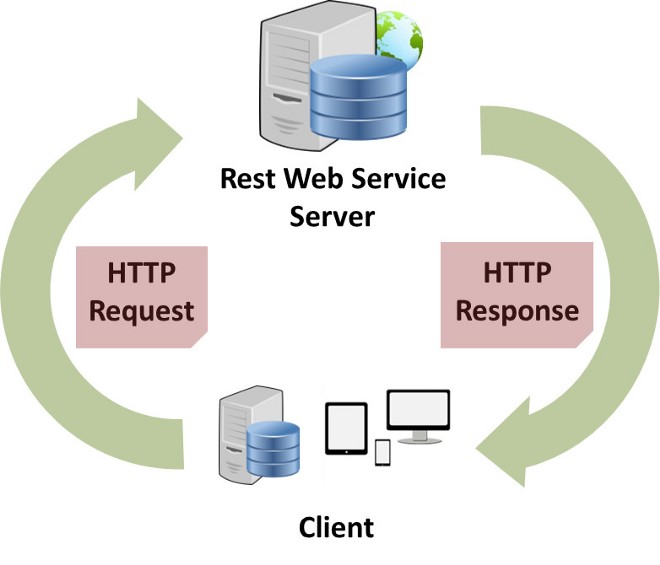
\includegraphics[width=0.5\linewidth]{images/design/clientserver.jpeg}}}%
    {\scriptsize%
     Source: \url{https://cdn-images-1.medium.com/max/660/1*EbBD6IXvf3o-YegUvRB_IA.jpeg}}
    \caption {A look at the server-client architecture with a RESTful interface.}
    \label{fig:design1}
\end{center}
\end{figure}

To demonstrate the functionality of the WebCure, we covered three different types of CRDTs used in AntidoteDB: a counter, a set and a multi-value register. We managed to support each of these data types on the server and the client as well.

\section{System's main components}

Let us have a look at the main components of the system:

\begin{figure}[!htb]
    \begin{center}
        \setlength{\fboxsep}{15pt}%
        \setlength{\fboxrule}{1pt}%
    \def\svgwidth{\linewidth}
    \fbox{\input{images/design/Main.pdf_tex}}
    \caption {A top-level view of the system's design.}
    \label{fig:design5}
\end{center}
\end{figure}

\subsection{Web Application}

First of all, in order for the user to be able to communicate with an AntidoteDB server, we are going to have a running web application that serves as a client. It runs in the web-browser, supports various commands from the user and sits on top of the local database layer. 

\vspace{5mm}For each of supported CRDTs, these are available commands:

\begin{itemize}
    \item \textit{read(key)} -- an asynchronous function that pulls database changes concerning the \textit{key} that the user passed.
         \begin{itemize}
         \item \textit{key}: a key to be read from the server's database;
         \item \textit{timestamp}: an optional parameter, which let us to set the timestamp at what the data should be read from;
     \end{itemize}
    \item \textit{update(key, op)}  -- an asynchronous function that processes user-made updates.
     \begin{itemize}
         \item \textit{key}: a key, which is going to be updated;
         \item \textit{op}: an operation, which is going to be performed on the key (it could differ depending on the data type it is running on);
     \end{itemize}
  \end{itemize}
  
 When a user tries to update the data on a client-side, there are two possibilities:
  
  \begin{itemize}
    \item{The request to the server is succesfull: in this case, the request would end up changing the data on the server's side, while the client will just update its own cache once it gets a response from the server.}
    \item{The request to the server is not succesfull: here, it is going to be a bit more interesting. We will have to wait for an error message and store the data in a temporary database for the updates that are not sent to the server's side just yet. Afterwards, I think it would be logical to have a timer, which will check the connection with the server. Once it is back, every transaction again is going to be sent to the server. After all the data is sent, this temporary database can be cleaned. }
\end{itemize}
    
    %TODO
    Several problems could arise, however, which we are going to discuss later.

\subsection{Server}

This part is an important part of the WebCure, as it provides the interface for the client and operates with the database layer as well. It supports the following scenarious for all the above-mentioned CRDTs:

\begin{itemize}
    \item receiving an operations or an array of operations performed on a CRDT-object, according to the key, and applying them on the server;
    \item sending back to the client the state of requested CRDT-object / objects according to their state on the server;
    %\item sending back states of all stored CRDT-objects, if a specific object was not asked for; 
\end{itemize}

\subsection{A database layer}

This layer should consist of the AntidoteDB database, which is going to store the actual states of CRDT-objects. When a user performs \textit{read} by \textit{key} operation from the cache, the following actions are taking place:

\begin{itemize}
\item Firstly, the state of the object \textit{\textbf{O}} is going to be found by \textit{\textbf{key}} in the database
\item Next, operations \textit{\textbf{o}} performed on the object \textit{\textbf{O}} are selected
\item Afterwards, selected operations \textit{\textbf{o}} applied on the object \textit{\textbf{O}}.
\item Finally, the object from the previous step is returned back as a response to the application.
\end{itemize} 


\begin{figure}[!htb]
    \begin{center}
    \def\svgwidth{\linewidth}
    \input{images/implementation/3tier.pdf_tex}
    \caption {3-Tier architecture.}
    \label{fig:dev1}
\end{center}
\end{figure}



\section{Offline functionality}

In this section, we are going to describe the offline functionality of the system.

Initially, the database is empty. Therefore, if the user is offline from the very beginning, he should be able to add the data into the database himself. 
The system represented in \figref*{fig:design5} will change by having only the Web Application and the database. However, whenever the connection is established with the server, the operations, which were stored in local database while offline, will be sent to the server. 

At the \figref*{fig:design6}, the sequence of getting the data from the local database is shown. This case describes the scenario, when the server is unavailable and the application has to read the value from the local database. 

\begin{figure}[!htb]
    \begin{center}
    \def\svgwidth{\columnwidth}
    \input{images/design/offlineProtocol.pdf_tex}
    \caption {Successful request of state from the local database -- Sequence diagram.}
    \label{fig:design6}
\end{center}
\end{figure}


\begin{figure}[!htb]
    \begin{center}
    \def\svgwidth{\columnwidth}
    \input{images/design/offlineStore.pdf_tex}
    \caption {Successful storing of an operation in the local database -- Sequence diagram.}
    \label{fig:design7}
\end{center}
\end{figure}

At the \textbf{Figure \ref{fig:design7}}, the sequence of storing the data locally is shown. When the connection is not there, the application will store in the database all offline-performed operations by the user. Afterwards, once the connection is re-established, that data will be sent back to the server. At the point when we read the state again from the server, the data, which is stored locally could be easily removed due to be pointless to hold on it. 


\section {Online functionality}

In this section, we are going to describe the online functionality of the system.



\section {The transition between offline and online modes}


\section{Optimization}